1. $y=\cfrac{|x+1|}{x+1}(x-1)=\begin{cases} x-1,\ x>-1,\\ 1-x,\ x<-1.\end{cases}$
$$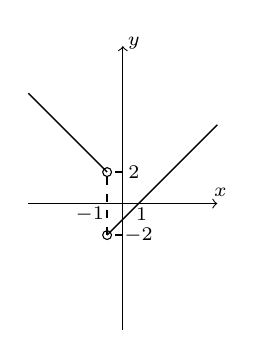
\begin{tikzpicture}[scale=0.2]
\tikzset {line01/.style={line width =0.5pt}}
\tikzset{line02/.style={line width =1pt}}
\tikzset{line03/.style={dashed,line width =0.5pt}}
%\filldraw [black] (0,0) circle (1pt);
\draw [->] (-6,0) -- (6,0);
\draw [->] (0,-8) -- (0,10);
\draw[line01] (-6,7) -- (-1,2);
\draw[line01] (-1,-2) -- (6,5);
\draw[line03] (-1,-2) -- (-1,2);
\draw[line03] (0,2) -- (-1,2);
\draw[line03] (0,-2) -- (-1,-2);
\draw (6.2,0.7) node {\scriptsize $x$};
\draw (1,-2) node {\scriptsize $-2$};
\draw (0.7,2) node {\scriptsize $2$};
\draw (1.2,-0.7) node {\scriptsize $1$};
\draw (-2.1,-0.7) node {\scriptsize $-1$};
\draw (0.7,10.2) node {\scriptsize $y$};
\draw (-1,2) circle (8pt);
\draw (-1,-2) circle (8pt);
\end{tikzpicture}$$
